\section{Overview}
\label{sec:overview}

\begin{figure}
\begin{verbatim}
var Color: int; // WHITE=1, GRAY=2, BLACK=3
\end{verbatim}
\begin{verbatim}
procedure TopWB(linear tid:Tid)
atomic [if (Color == WHITE) Color := GRAY];
{
  var cNoLock:int;
  cNoLock := GetColorNoLock(tid);
  call YieldColorsGetDarker(); 
  if (cNoLock == WHITE) 
    call MidWB(tid);
}
\end{verbatim}
\begin{verbatim}
procedure MidWB(linear tid:Tid)
atomic [if (Color == WHITE) Color := GRAY];
{
  var cLock:int;
  call AcquireLock(tid);
  cLock := GetColorLocked(tid);
  if (cLock == WHITE) 
    call SetColorLocked(tid, GRAY);
  call ReleaseLock(tid);
}
\end{verbatim}
\begin{verbatim}
procedure YieldColorsGetDarker()
ensures Color >= old(Color);
{
  yield Color >= old(Color);
}
\end{verbatim}
\begin{verbatim}
procedure GetColorNoLock(linear tid:Tid) 
  returns (cl:int) atomic [...];
procedure AcquireLock(linear tid:Tid) 
  right [...];
procedure ReleaseLock(linear tid:Tid) 
  left [...];
procedure GetColorLocked(linear tid:Tid) 
  returns (cl:int) both [...];
procedure SetColorLocked(linear tid:Tid, 
  cl: int) atomic [...];
\end{verbatim}
\caption{Write barrier}
\label{fig:reft}
\end{figure}

\civl supports the verification of refinement of atomic action specifications for procedures. 
We illustrate this technique on the proram in Figure~\ref{fig:reft},
a simplified version of the write barrier in a concurrent garbage collector (GC).
In a concurrent GC, a color (either \exC{WHITE}, \exC{GRAY}, or \exC{BLACK})
is associated with each object on the heap.  
Before writing to an address \exC{addr}, a mutator thread checks 
if color associated with \exC{addr} is \exC{WHITE}
and sets it to \exC{GRAY}, indicating that the object at this address
and objects reachable from it should not be garbage collected. 

Procedure \exC{TopWB} implements the write barrier.
To simplify the exposition, 
we consider only a single object whose color is stored in the shared variable \exC{Color}.
To avoid the cost of locking for each address encountered, \exC{TopWB} reads \exC{Color} without holding a lock.
If the color is {\tt WHITE}, it calls the more expensive procedure \exC{MidWB} 
that re-examines and possibly updates \exC{Color} while holding the lock.
\civl simplifies reasoning about \exC{TopWB} and \exC{MidWB} by allowing us to 
compactly express their specification as the following atomic action:
\begin{verbatim}
[if (Color == WHITE) Color := GRAY]
\end{verbatim}
This specification indicates that regardless of the different implementations of 
\exC{TopWB} and \exC{MidWB} and regardless of how the environment interferes
with their execution, to their respective callers it appears as if they atomically execute the above code.

The correctness of \exC{TopWB} is not obvious.
Consider the following potential scenario. 
\exC{TopWB}, not holding a lock, reads {\tt Color} and
sets \exC{cNoLock} to \exC{GRAY} and then yields inside the call to
\exC{YieldColorsGetDarker}. Another thread sets {\tt Color} to
{\tt WHITE}. \exC{TopWB} resumes, but does nothing and exits,
because the procedure-local variable \exC{cNoLock} is \exC{GRAY}. In this scenario, the atomic action
specification of \exC{TopWB} would not be satisfied. However, in the GC this
scenario is not possible. 
The yield predicate in \exC{YieldColorsGetDarker} expresses the fact that
other threads in the environment of the thread running \exC{TopWB} can
only modify {\tt Color} to a higher (darker) value. 
\civl then verifies that, for every control path through \exC{TopWB}
procedure, exactly one {\tt yield}-to-{\tt yield} execution
fragment implements the atomic action specification and that other fragments do not modify
global state. 
This proof requires both correct modeling of environment interference in \exC{YieldColorsGetDarker}
and the atomic action specification for the called procedure \exC{MidWB}.
The \civl verifier automatically computes a logical verification condition capturing
this proof obligation from the body and specification of \exC{TopWB}.
Just as the verification of \exC{TopWB} builds on the specification of \exC{MidWB},
the verification of \exC{MidWB} builds on other refinement proofs (not shown) 
of the procedures called in \exC{MidWB};
these called procedures are shown at the bottom of the figure. 

There are two important benefits of atomic action specifications.
First, an atomic action is often the most compact and precise way to express the specification a procedure.
Second, an atomic action specification successfully hides from the caller of a procedure $P$
the potentially numerous yields inside the body of $P$.
This capability provides modularity akin to that provided by the frame rule for sequential programs.
Without this capability, any postcondition $\phi$ needed by the caller of $P$ must be made explicit in the precondition 
and yield predicates of $P$ and all procedures recursively called inside it.
With this capability, the caller achieves the same effect by writing $\yield{\phi}$ before and after the call, 
provided that $\phi$ is preserved by the atomic action specification of $P$.

As explained above, the refinement checking is performed on cooperative semantics in which a 
{\tt yield}-to-{\tt yield} execution fragment of code is executed atomically.
However, in a real execution, control can switch between threads at any point in the code. 
A naive modeling of a real execution would put a yield statement before every instruction in the code.
The absence of a yield statement before every instruction is justified by reasoning about mover types~\cite{FlanaganFLQ08}. 

The procedures called in \exC{MidWB} have the mover types claimed in their
declarations and verified by \civl. 
For example, the mover type of \exC{Acquirelock} is {\tt right} which indicates 
that it commutes later in time against concurrently executing environment actions.
\exC{ReleaseLock} has mover type {\tt left} and it commutes earlier in time;
\exC{SetColorLocked} has mover type {\tt atomic} and it does not commute;
\exC{GetColorLocked} has mover type {\tt both} and it commutes both earlier and later in time.
These mover types are checked by constructing verification conditions from each pair of atomic actions.

Note that \civl allows the programmer to avoid mover reasoning by eschewing
the mover types {\tt right}, {\tt left}, and {\tt both}.
In this case, the only mover type is {\tt atomic} which does not require any verification.
The tradeoff is that a yield statement accompanied with an appropriate assertion
must be inserted before every invocation of an atomic action.
We have observed that in many concurrent programs, this tradeoff is inappropriate for two reasons.
First, the annotation burden goes up because sophisticated ghost variables may need to be introduced in the 
program semantics.\footnote{Well-scoped location invariants that cannot refer to the state of other threads are known to be incomplete, 
both in theory and in practice.}
Second, the cost of the pairwise mover reasoning is replaced by the cost of pairwise non-interference checks between yield assertions 
and concurrently executing atomic actions.

\begin{figure}
\begin{center}
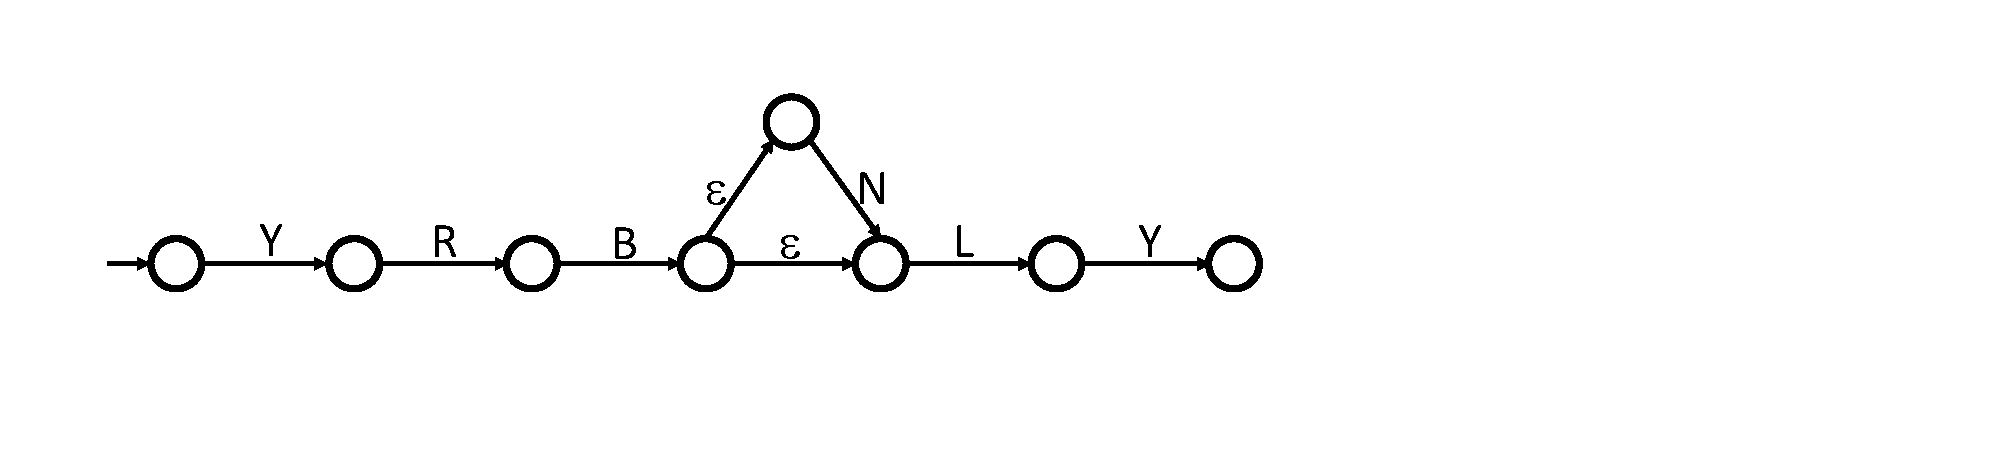
\includegraphics[scale=0.35]{MidWB.pdf}
\end{center}
\caption{Abstraction of \exC{MidWB}}
\label{fig:midwb}
\end{figure}

\begin{figure}
\begin{center}
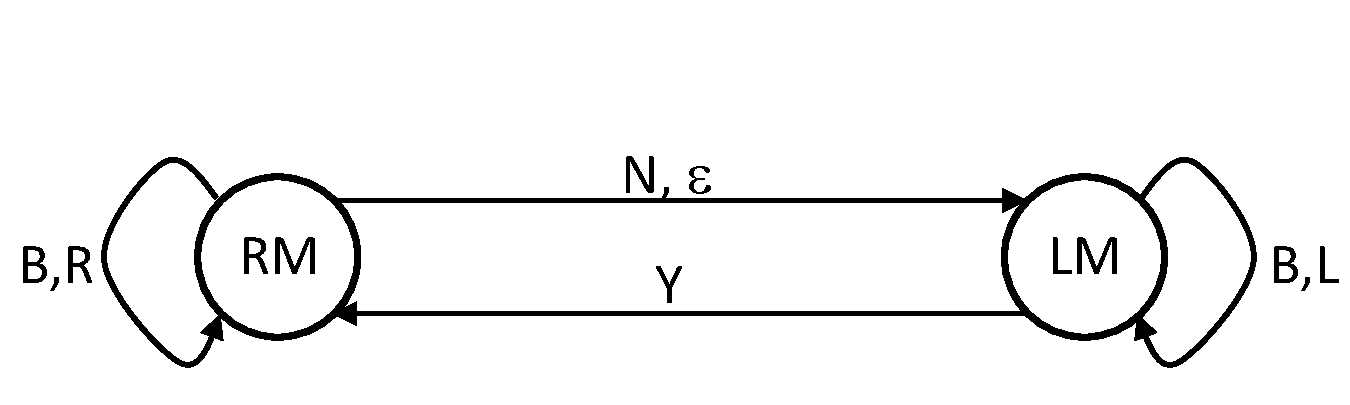
\includegraphics[scale=0.35]{YieldTypeCheckingAutomaton.pdf}
\end{center}
\caption{Yield sufficiency automaton ($YSA$)}
\label{fig:ysa}
\end{figure}

Finally, given the mover types of atomic action specifications, the \civl verifier ensures
that the absence of yields is justified by constructing an abstraction of \exC{MidWB} 
that interprets each atomic action invoked by \exC{MidWB} according to its mover type.
This abstraction is shown in Figure~\ref{fig:midwb}.
The edge labels belong to the set $\{B,R,L,N,Y\}$, where $B$ (both mover), $R$ (right mover), $L$ (left mover), and $N$ (non mover) 
represent the various kinds of atomic actions described earlier, and $Y$ represents a yield statement.
Note that there are implicit yield statements at the beginning and end of the body of each procedure.

The \civl verifier checks that this automaton is simulated by the {\em Yield Sufficiency Automaton\/} ($\YSA$ in Figure~\ref{fig:ysa})
using an existing algorithm for computing simulation relation~\cite{HenzingerHK95}.
The $\YSA$ automaton encodes all sequences of atomic actions and yields for which safety of cooperative semantics is sufficient 
for safety of preemptive semantics.
This automaton has two states, $\RM$ and $\LM$,
and allows traces in which {\em transactions\/} are separated by yields.
Each transaction starts with a sequence of right movers (or both movers) and ends with a sequence of left movers (or both movers).
In the middle, it can have at most one non mover.

The atomic action specification of \exC{MidWB} makes no reference to the lock variable, 
although its implementation involves a lock. 
When verifying refinement for \exC{MidWB}, the lock variable has been hidden. 
\civl allows the programmer to both introduce and hide variables in each refinement step,
thereby providing the capability to perform data refinement.
The ability to introduce and hide variables and write yield predicates specific to each refinement step 
facilitates proofs spanning large abstraction gaps between the specification and implementation.
